\chapter{Additional Studies}
\label{chap:Additional Studies}

\begin{figure}
    \centering
    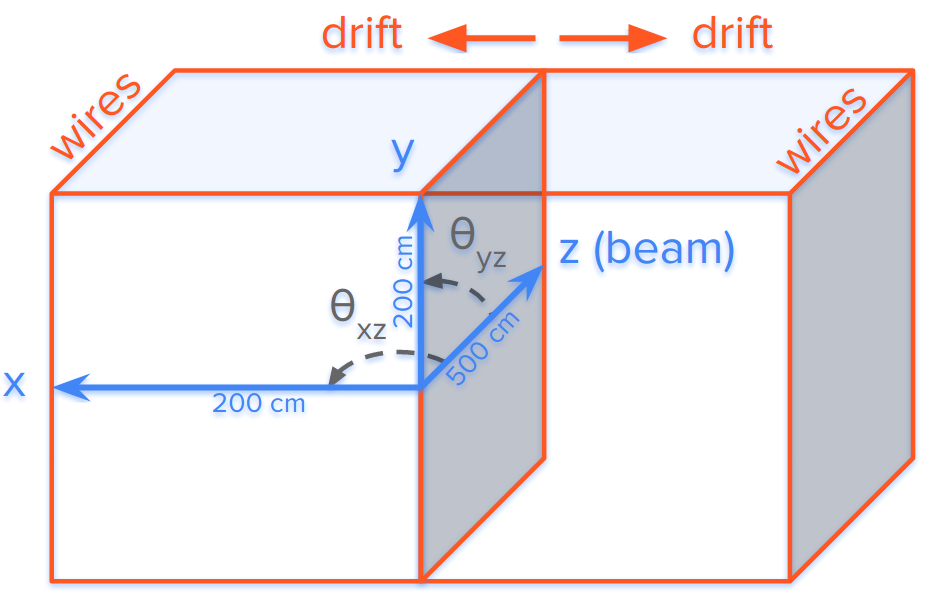
\includegraphics[width =\largefigwidth]{Figures/SBND_geometry.png}
    \caption{The SBND coordinate system showing the definition of the $\theta_{XZ}$ and $\theta_{YZ}$ angles.}
    \label{fig:my_label}
\end{figure}


\begin{figure}
    \centering
    \fbox{Reco efficiency vs XZ angle (Y is fixed at 0m)}
    \caption{}
    \label{fig:my_label}
\end{figure}

\begin{figure}
    \centering
    \fbox{Reco efficiency vs XY angle (Z is fixed at 2.5m)}
    \caption{Caption}
    \label{fig:my_label}
\end{figure}

\begin{figure}
    \centering
    \fbox{Reco efficiency vs true deposited energy}
    \caption{Caption}
    \label{fig:my_label}
\end{figure}

\begin{figure}
    \centering
    \fbox{Fractional resolution of \electron $\pi^+$ with lower (no?) hit thresholding.}
    \caption{Caption}
    \label{fig:my_label}
\end{figure}

\begin{figure}
    \centering
    \fbox{Validation with some sort of low energy sample (supernova neutrinos?)}
    \caption{Caption}
    \label{fig:my_label}
\end{figure}



